% Options for packages loaded elsewhere
\PassOptionsToPackage{unicode}{hyperref}
\PassOptionsToPackage{hyphens}{url}
%
\documentclass[
]{article}
\usepackage{amsmath,amssymb}
\usepackage{iftex}
\ifPDFTeX
  \usepackage[T1]{fontenc}
  \usepackage[utf8]{inputenc}
  \usepackage{textcomp} % provide euro and other symbols
\else % if luatex or xetex
  \usepackage{unicode-math} % this also loads fontspec
  \defaultfontfeatures{Scale=MatchLowercase}
  \defaultfontfeatures[\rmfamily]{Ligatures=TeX,Scale=1}
\fi
\usepackage{lmodern}
\ifPDFTeX\else
  % xetex/luatex font selection
\fi
% Use upquote if available, for straight quotes in verbatim environments
\IfFileExists{upquote.sty}{\usepackage{upquote}}{}
\IfFileExists{microtype.sty}{% use microtype if available
  \usepackage[]{microtype}
  \UseMicrotypeSet[protrusion]{basicmath} % disable protrusion for tt fonts
}{}
\makeatletter
\@ifundefined{KOMAClassName}{% if non-KOMA class
  \IfFileExists{parskip.sty}{%
    \usepackage{parskip}
  }{% else
    \setlength{\parindent}{0pt}
    \setlength{\parskip}{6pt plus 2pt minus 1pt}}
}{% if KOMA class
  \KOMAoptions{parskip=half}}
\makeatother
\usepackage{xcolor}
\usepackage[margin=1in]{geometry}
\usepackage{color}
\usepackage{fancyvrb}
\newcommand{\VerbBar}{|}
\newcommand{\VERB}{\Verb[commandchars=\\\{\}]}
\DefineVerbatimEnvironment{Highlighting}{Verbatim}{commandchars=\\\{\}}
% Add ',fontsize=\small' for more characters per line
\usepackage{framed}
\definecolor{shadecolor}{RGB}{248,248,248}
\newenvironment{Shaded}{\begin{snugshade}}{\end{snugshade}}
\newcommand{\AlertTok}[1]{\textcolor[rgb]{0.94,0.16,0.16}{#1}}
\newcommand{\AnnotationTok}[1]{\textcolor[rgb]{0.56,0.35,0.01}{\textbf{\textit{#1}}}}
\newcommand{\AttributeTok}[1]{\textcolor[rgb]{0.13,0.29,0.53}{#1}}
\newcommand{\BaseNTok}[1]{\textcolor[rgb]{0.00,0.00,0.81}{#1}}
\newcommand{\BuiltInTok}[1]{#1}
\newcommand{\CharTok}[1]{\textcolor[rgb]{0.31,0.60,0.02}{#1}}
\newcommand{\CommentTok}[1]{\textcolor[rgb]{0.56,0.35,0.01}{\textit{#1}}}
\newcommand{\CommentVarTok}[1]{\textcolor[rgb]{0.56,0.35,0.01}{\textbf{\textit{#1}}}}
\newcommand{\ConstantTok}[1]{\textcolor[rgb]{0.56,0.35,0.01}{#1}}
\newcommand{\ControlFlowTok}[1]{\textcolor[rgb]{0.13,0.29,0.53}{\textbf{#1}}}
\newcommand{\DataTypeTok}[1]{\textcolor[rgb]{0.13,0.29,0.53}{#1}}
\newcommand{\DecValTok}[1]{\textcolor[rgb]{0.00,0.00,0.81}{#1}}
\newcommand{\DocumentationTok}[1]{\textcolor[rgb]{0.56,0.35,0.01}{\textbf{\textit{#1}}}}
\newcommand{\ErrorTok}[1]{\textcolor[rgb]{0.64,0.00,0.00}{\textbf{#1}}}
\newcommand{\ExtensionTok}[1]{#1}
\newcommand{\FloatTok}[1]{\textcolor[rgb]{0.00,0.00,0.81}{#1}}
\newcommand{\FunctionTok}[1]{\textcolor[rgb]{0.13,0.29,0.53}{\textbf{#1}}}
\newcommand{\ImportTok}[1]{#1}
\newcommand{\InformationTok}[1]{\textcolor[rgb]{0.56,0.35,0.01}{\textbf{\textit{#1}}}}
\newcommand{\KeywordTok}[1]{\textcolor[rgb]{0.13,0.29,0.53}{\textbf{#1}}}
\newcommand{\NormalTok}[1]{#1}
\newcommand{\OperatorTok}[1]{\textcolor[rgb]{0.81,0.36,0.00}{\textbf{#1}}}
\newcommand{\OtherTok}[1]{\textcolor[rgb]{0.56,0.35,0.01}{#1}}
\newcommand{\PreprocessorTok}[1]{\textcolor[rgb]{0.56,0.35,0.01}{\textit{#1}}}
\newcommand{\RegionMarkerTok}[1]{#1}
\newcommand{\SpecialCharTok}[1]{\textcolor[rgb]{0.81,0.36,0.00}{\textbf{#1}}}
\newcommand{\SpecialStringTok}[1]{\textcolor[rgb]{0.31,0.60,0.02}{#1}}
\newcommand{\StringTok}[1]{\textcolor[rgb]{0.31,0.60,0.02}{#1}}
\newcommand{\VariableTok}[1]{\textcolor[rgb]{0.00,0.00,0.00}{#1}}
\newcommand{\VerbatimStringTok}[1]{\textcolor[rgb]{0.31,0.60,0.02}{#1}}
\newcommand{\WarningTok}[1]{\textcolor[rgb]{0.56,0.35,0.01}{\textbf{\textit{#1}}}}
\usepackage{graphicx}
\makeatletter
\def\maxwidth{\ifdim\Gin@nat@width>\linewidth\linewidth\else\Gin@nat@width\fi}
\def\maxheight{\ifdim\Gin@nat@height>\textheight\textheight\else\Gin@nat@height\fi}
\makeatother
% Scale images if necessary, so that they will not overflow the page
% margins by default, and it is still possible to overwrite the defaults
% using explicit options in \includegraphics[width, height, ...]{}
\setkeys{Gin}{width=\maxwidth,height=\maxheight,keepaspectratio}
% Set default figure placement to htbp
\makeatletter
\def\fps@figure{htbp}
\makeatother
\setlength{\emergencystretch}{3em} % prevent overfull lines
\providecommand{\tightlist}{%
  \setlength{\itemsep}{0pt}\setlength{\parskip}{0pt}}
\setcounter{secnumdepth}{-\maxdimen} % remove section numbering
\ifLuaTeX
  \usepackage{selnolig}  % disable illegal ligatures
\fi
\IfFileExists{bookmark.sty}{\usepackage{bookmark}}{\usepackage{hyperref}}
\IfFileExists{xurl.sty}{\usepackage{xurl}}{} % add URL line breaks if available
\urlstyle{same}
\hypersetup{
  pdftitle={Tarea Betamétrica},
  pdfauthor={Richard Guanoluisa},
  hidelinks,
  pdfcreator={LaTeX via pandoc}}

\title{Tarea Betamétrica}
\author{Richard Guanoluisa}
\date{2023-11-06}

\begin{document}
\maketitle

\hypertarget{carga-libreruxedas}{%
\section{Carga librerías}\label{carga-libreruxedas}}

\begin{Shaded}
\begin{Highlighting}[]
\FunctionTok{library}\NormalTok{(openxlsx)}
\FunctionTok{library}\NormalTok{(dplyr)}
\end{Highlighting}
\end{Shaded}

\begin{verbatim}
## 
## Attaching package: 'dplyr'
\end{verbatim}

\begin{verbatim}
## The following objects are masked from 'package:stats':
## 
##     filter, lag
\end{verbatim}

\begin{verbatim}
## The following objects are masked from 'package:base':
## 
##     intersect, setdiff, setequal, union
\end{verbatim}

\begin{Shaded}
\begin{Highlighting}[]
\FunctionTok{library}\NormalTok{(ggplot2)}
\FunctionTok{library}\NormalTok{(fdth)}
\end{Highlighting}
\end{Shaded}

\begin{verbatim}
## 
## Attaching package: 'fdth'
\end{verbatim}

\begin{verbatim}
## The following objects are masked from 'package:stats':
## 
##     sd, var
\end{verbatim}

\begin{Shaded}
\begin{Highlighting}[]
\FunctionTok{library}\NormalTok{(stringr)}
\FunctionTok{library}\NormalTok{(stargazer)}
\end{Highlighting}
\end{Shaded}

\begin{verbatim}
## 
## Please cite as:
\end{verbatim}

\begin{verbatim}
##  Hlavac, Marek (2022). stargazer: Well-Formatted Regression and Summary Statistics Tables.
\end{verbatim}

\begin{verbatim}
##  R package version 5.2.3. https://CRAN.R-project.org/package=stargazer
\end{verbatim}

\begin{Shaded}
\begin{Highlighting}[]
\FunctionTok{library}\NormalTok{(lmtest)}
\end{Highlighting}
\end{Shaded}

\begin{verbatim}
## Loading required package: zoo
\end{verbatim}

\begin{verbatim}
## 
## Attaching package: 'zoo'
\end{verbatim}

\begin{verbatim}
## The following objects are masked from 'package:base':
## 
##     as.Date, as.Date.numeric
\end{verbatim}

\hypertarget{carga-datos}{%
\section{Carga datos}\label{carga-datos}}

\begin{Shaded}
\begin{Highlighting}[]
\CommentTok{\# Cargar datos en datos\_db}
\NormalTok{datos\_db }\OtherTok{\textless{}{-}} \FunctionTok{read.xlsx}\NormalTok{(}\StringTok{"C:}\SpecialCharTok{\textbackslash{}\textbackslash{}}\StringTok{Users}\SpecialCharTok{\textbackslash{}\textbackslash{}}\StringTok{Richard}\SpecialCharTok{\textbackslash{}\textbackslash{}}\StringTok{Documents}\SpecialCharTok{\textbackslash{}\textbackslash{}}\StringTok{DOCS RICHARD}\SpecialCharTok{\textbackslash{}\textbackslash{}}\StringTok{Cursos}\SpecialCharTok{\textbackslash{}\textbackslash{}}\StringTok{2023 Reto betametrica/empresas\_HEBM18.xlsx"}\NormalTok{,}\AttributeTok{na.strings =}\NormalTok{ T)}
\CommentTok{\# Filtrar datos completos}
\NormalTok{datos\_db }\OtherTok{\textless{}{-}}\NormalTok{ datos\_db }\SpecialCharTok{\%\textgreater{}\%} 
  \FunctionTok{filter}\NormalTok{(}\FunctionTok{complete.cases}\NormalTok{(.))}
\end{Highlighting}
\end{Shaded}

\hypertarget{realizar-un-gruxe1fico-de-barras-considerando-las-empresas-de-la-regiuxf3n-sierra}{%
\section{1. Realizar un gráfico de barras considerando las empresas de
la región
SIERRA}\label{realizar-un-gruxe1fico-de-barras-considerando-las-empresas-de-la-regiuxf3n-sierra}}

\begin{Shaded}
\begin{Highlighting}[]
\CommentTok{\# Resumen del conjunto de datos}
\FunctionTok{summary}\NormalTok{(datos\_db)}
\end{Highlighting}
\end{Shaded}

\begin{verbatim}
##      2019               2018                PR             EXPEDIENTE       
##  Length:19121       Length:19121       Length:19121       Length:19121      
##  Class :character   Class :character   Class :character   Class :character  
##  Mode  :character   Mode  :character   Mode  :character   Mode  :character  
##                                                                             
##                                                                             
##                                                                             
##     NOMBRE          TIPO.COMPAÑIA      ACTIVIDAD.ECONÓMICA    REGIÓN         
##  Length:19121       Length:19121       Length:19121        Length:19121      
##  Class :character   Class :character   Class :character    Class :character  
##  Mode  :character   Mode  :character   Mode  :character    Mode  :character  
##                                                                              
##                                                                              
##                                                                              
##   PROVINCIA            CIUDAD             TAMAÑO             SECTOR         
##  Length:19121       Length:19121       Length:19121       Length:19121      
##  Class :character   Class :character   Class :character   Class :character  
##  Mode  :character   Mode  :character   Mode  :character   Mode  :character  
##                                                                             
##                                                                             
##                                                                             
##  CANT..EMPLEADOS        ACTIVO            PATRIMONIO       INGRESOS.POR.VENTA
##  Min.   :    0.00   Min.   :        0   Min.   :-9926290   Min.   :      0   
##  1st Qu.:    4.00   1st Qu.:    75428   1st Qu.:   12690   1st Qu.: 137470   
##  Median :    6.00   Median :   187096   Median :   46851   Median : 250184   
##  Mean   :   12.78   Mean   :   561708   Mean   :  233994   Mean   : 321552   
##  3rd Qu.:   10.00   3rd Qu.:   428543   3rd Qu.:  139405   3rd Qu.: 465833   
##  Max.   :22008.00   Max.   :243754719   Max.   :64080222   Max.   :4448772   
##     UTILIDAD            INGRESOS      
##  Min.   :-973982.2   Min.   :      0  
##  1st Qu.:    789.9   1st Qu.: 137470  
##  Median :   7628.3   Median : 250184  
##  Mean   :  26786.3   Mean   : 321552  
##  3rd Qu.:  22872.4   3rd Qu.: 465833  
##  Max.   : 994057.8   Max.   :4448772
\end{verbatim}

\begin{Shaded}
\begin{Highlighting}[]
\CommentTok{\# Asignar datos limpios y filtrados a new\_db}
\NormalTok{new\_db }\OtherTok{\textless{}{-}}\NormalTok{ datos\_db }\SpecialCharTok{\%\textgreater{}\%} 
  \FunctionTok{select}\NormalTok{(NOMBRE,REGIÓN,PROVINCIA,INGRESOS,CANT..EMPLEADOS,UTILIDAD,CIUDAD) }\SpecialCharTok{\%\textgreater{}\%} 
  \FunctionTok{filter}\NormalTok{(REGIÓN }\SpecialCharTok{==} \StringTok{"SIERRA"}\NormalTok{)}
\CommentTok{\# Reducción de valores}
\NormalTok{new\_db}\SpecialCharTok{$}\NormalTok{INGRESOS }\OtherTok{\textless{}{-}}\NormalTok{ new\_db}\SpecialCharTok{$}\NormalTok{INGRESOS}\SpecialCharTok{/}\DecValTok{1000}
\CommentTok{\# Histograma de Ingresos }
\FunctionTok{summary}\NormalTok{(new\_db}\SpecialCharTok{$}\NormalTok{INGRESOS)}
\end{Highlighting}
\end{Shaded}

\begin{verbatim}
##    Min. 1st Qu.  Median    Mean 3rd Qu.    Max. 
##     0.0   142.2   258.0   326.3   471.5  2994.4
\end{verbatim}

\begin{Shaded}
\begin{Highlighting}[]
\NormalTok{tabla\_frecuencia }\OtherTok{\textless{}{-}} \FunctionTok{fdt}\NormalTok{(new\_db}\SpecialCharTok{$}\NormalTok{INGRESOS,}\AttributeTok{start =} \DecValTok{10}\NormalTok{,}\AttributeTok{end =} \DecValTok{100}\NormalTok{,}\AttributeTok{h=}\DecValTok{10}\NormalTok{)}
\NormalTok{tabla\_frecuencia1 }\OtherTok{\textless{}{-}} \FunctionTok{data.frame}\NormalTok{(tabla\_frecuencia}\SpecialCharTok{$}\NormalTok{table)}
\NormalTok{tabla\_frecuencia1}\SpecialCharTok{$}\NormalTok{rango }\OtherTok{\textless{}{-}} \FunctionTok{seq}\NormalTok{(}\DecValTok{20}\NormalTok{,}\DecValTok{100}\NormalTok{,}\DecValTok{10}\NormalTok{)}
\NormalTok{tabla\_frecuencia1}\SpecialCharTok{$}\NormalTok{cf... }\OtherTok{\textless{}{-}} \FunctionTok{round}\NormalTok{(tabla\_frecuencia1}\SpecialCharTok{$}\NormalTok{cf...,}\DecValTok{0}\NormalTok{)}
\FunctionTok{View}\NormalTok{(tabla\_frecuencia1)}
\CommentTok{\# Gráfico del histograma }
\NormalTok{g1 }\OtherTok{\textless{}{-}} \FunctionTok{ggplot}\NormalTok{(}\AttributeTok{data =}\NormalTok{ tabla\_frecuencia1,}
       \FunctionTok{aes}\NormalTok{(}\AttributeTok{x=}\FunctionTok{seq}\NormalTok{(}\DecValTok{10}\NormalTok{,}\DecValTok{90}\NormalTok{,}\DecValTok{10}\NormalTok{),}
           \AttributeTok{y=}\NormalTok{f)) }\SpecialCharTok{+} 
  \FunctionTok{geom\_bar}\NormalTok{(}\AttributeTok{stat =} \StringTok{"identity"}\NormalTok{,}\AttributeTok{fill=}\StringTok{"royalblue"}\NormalTok{)}\SpecialCharTok{+}
  \FunctionTok{geom\_text}\NormalTok{(}\FunctionTok{aes}\NormalTok{(}\AttributeTok{label=}\NormalTok{f),}\AttributeTok{position=}\StringTok{"identity"}\NormalTok{,}\AttributeTok{vjust=}\DecValTok{0}\NormalTok{,}\AttributeTok{size=}\DecValTok{6}\NormalTok{)}\SpecialCharTok{+}
  \FunctionTok{scale\_x\_continuous}\NormalTok{(}\AttributeTok{breaks =}\NormalTok{ tabla\_frecuencia1}\SpecialCharTok{$}\NormalTok{rango)}\SpecialCharTok{+}
  \FunctionTok{theme}\NormalTok{(}\AttributeTok{axis.text.x =} \FunctionTok{element\_text}\NormalTok{(}\AttributeTok{size =} \DecValTok{12}\NormalTok{,}\AttributeTok{angle =} \DecValTok{90}\NormalTok{))}\SpecialCharTok{+}
  \FunctionTok{labs}\NormalTok{(}\AttributeTok{title =} \StringTok{"Frecuencia absoluta de los ingresos anuales"}\NormalTok{,}\AttributeTok{subtitle =} \StringTok{"Pequeñas empresas de la Sierra del Ecuador"}\NormalTok{)}\SpecialCharTok{+}
  \FunctionTok{xlab}\NormalTok{(}\StringTok{"Ingresos por rango en miles"}\NormalTok{)}\SpecialCharTok{+}
  \FunctionTok{ylab}\NormalTok{(}\StringTok{"Número de empresas"}\NormalTok{)}
\NormalTok{g1}
\end{Highlighting}
\end{Shaded}

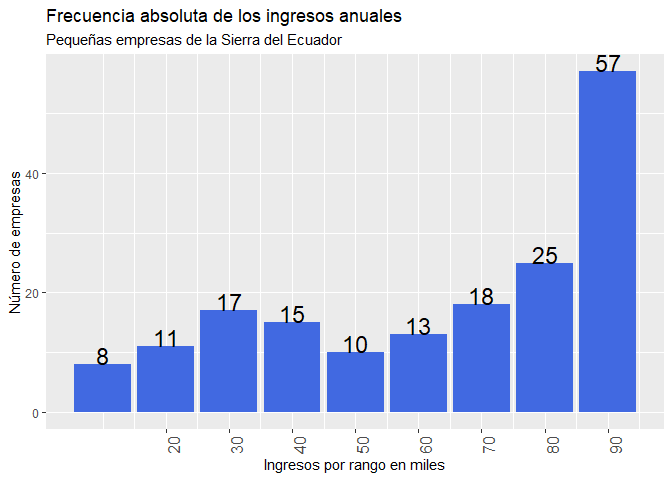
\includegraphics{Tarea-Betamétrica_files/figure-latex/unnamed-chunk-3-1.pdf}

\hypertarget{realiza-una-regresiuxf3n-simple-que-explique-el-ingreso-en-funciuxf3n-de-la-cantidad-de-empleados.-para-efectos-del-ejercicio-se-debe-filtrar-los-casos-cuyo-ingreso-y-cantidad-de-empleados-sea-igual-a-0.-la-regresiuxf3n-suxf3lo-debe-construirse-usando-la-provincia-del-guayas.-se-debe-reportar-los-resultados-la-interpretaciuxf3n-de-los-coeficientes-las-pruebas-de-autocorrelaciuxf3n-heterocedasticidad.}{%
\section{2. Realiza una regresión simple que explique el ingreso en
función de la cantidad de empleados. Para efectos del ejercicio, se debe
filtrar los casos cuyo ingreso y cantidad de empleados sea igual a 0. La
regresión sólo debe construirse usando la provincia del Guayas. Se debe
reportar los resultados, la interpretación de los coeficientes, las
pruebas de autocorrelación,
heterocedasticidad.}\label{realiza-una-regresiuxf3n-simple-que-explique-el-ingreso-en-funciuxf3n-de-la-cantidad-de-empleados.-para-efectos-del-ejercicio-se-debe-filtrar-los-casos-cuyo-ingreso-y-cantidad-de-empleados-sea-igual-a-0.-la-regresiuxf3n-suxf3lo-debe-construirse-usando-la-provincia-del-guayas.-se-debe-reportar-los-resultados-la-interpretaciuxf3n-de-los-coeficientes-las-pruebas-de-autocorrelaciuxf3n-heterocedasticidad.}}

\begin{Shaded}
\begin{Highlighting}[]
\CommentTok{\# Directorio}
\FunctionTok{setwd}\NormalTok{(}\StringTok{"C:}\SpecialCharTok{\textbackslash{}\textbackslash{}}\StringTok{Users}\SpecialCharTok{\textbackslash{}\textbackslash{}}\StringTok{Richard}\SpecialCharTok{\textbackslash{}\textbackslash{}}\StringTok{Documents}\SpecialCharTok{\textbackslash{}\textbackslash{}}\StringTok{DOCS RICHARD}\SpecialCharTok{\textbackslash{}\textbackslash{}}\StringTok{Cursos}\SpecialCharTok{\textbackslash{}\textbackslash{}}\StringTok{2023 Reto betametrica}\SpecialCharTok{\textbackslash{}\textbackslash{}}\StringTok{Tarea Betamétrica/"}\NormalTok{)}
\CommentTok{\# Archivo}
\NormalTok{db\_r }\OtherTok{\textless{}{-}}\NormalTok{ openxlsx}\SpecialCharTok{::}\FunctionTok{read.xlsx}\NormalTok{(}\StringTok{"empresas\_HEBM18.xlsx"}\NormalTok{)}
\CommentTok{\# asginar datos filtrados a db\_r}
\NormalTok{db\_r\_fil }\OtherTok{\textless{}{-}}\NormalTok{ db\_r }\SpecialCharTok{\%\textgreater{}\%} 
  \FunctionTok{select}\NormalTok{(PROVINCIA,INGRESOS,CANT..EMPLEADOS) }\SpecialCharTok{\%\textgreater{}\%} 
  \FunctionTok{filter}\NormalTok{(INGRESOS}\SpecialCharTok{\textgreater{}}\DecValTok{0} \SpecialCharTok{\&}\NormalTok{ CANT..EMPLEADOS}\SpecialCharTok{\textgreater{}}\DecValTok{0} \SpecialCharTok{\&}\NormalTok{ PROVINCIA}\SpecialCharTok{==} \StringTok{"GUAYAS                                            "}\NormalTok{)}
\NormalTok{db\_r\_fil\_1 }\OtherTok{\textless{}{-}}\NormalTok{ db\_r\_fil }\SpecialCharTok{\%\textgreater{}\%} 
  \FunctionTok{select}\NormalTok{(INGRESOS,CANT..EMPLEADOS)}
\FunctionTok{summary}\NormalTok{(db\_r\_fil\_1)}
\end{Highlighting}
\end{Shaded}

\begin{verbatim}
##     INGRESOS       CANT..EMPLEADOS   
##  Min.   :    301   Min.   :    1.00  
##  1st Qu.: 160883   1st Qu.:    4.00  
##  Median : 277955   Median :    6.00  
##  Mean   : 354438   Mean   :   15.78  
##  3rd Qu.: 493443   3rd Qu.:    9.00  
##  Max.   :4448772   Max.   :22008.00
\end{verbatim}

\begin{Shaded}
\begin{Highlighting}[]
\NormalTok{modelo }\OtherTok{\textless{}{-}} \FunctionTok{lm}\NormalTok{(INGRESOS}\SpecialCharTok{\textasciitilde{}}\NormalTok{.,}\AttributeTok{data =}\NormalTok{ db\_r\_fil\_1)}
\FunctionTok{summary}\NormalTok{(modelo)}
\end{Highlighting}
\end{Shaded}

\begin{verbatim}
## 
## Call:
## lm(formula = INGRESOS ~ ., data = db_r_fil_1)
## 
## Residuals:
##     Min      1Q  Median      3Q     Max 
## -439268 -193574  -76563  138947 4093811 
## 
## Coefficients:
##                  Estimate Std. Error t value Pr(>|t|)    
## (Intercept)     3.541e+05  3.028e+03  116.94   <2e-16 ***
## CANT..EMPLEADOS 1.852e+01  9.357e+00    1.98   0.0478 *  
## ---
## Signif. codes:  0 '***' 0.001 '**' 0.01 '*' 0.05 '.' 0.1 ' ' 1
## 
## Residual standard error: 248200 on 6732 degrees of freedom
## Multiple R-squared:  0.0005818,  Adjusted R-squared:  0.0004333 
## F-statistic: 3.919 on 1 and 6732 DF,  p-value: 0.04779
\end{verbatim}

\begin{Shaded}
\begin{Highlighting}[]
\CommentTok{\#ingresos = intercepto +b * cant empleado +error}
\CommentTok{\#ingresos = 3.541+1.852*cant empleados}
\CommentTok{\#Gráficos}
\NormalTok{grafico1}\OtherTok{=}\FunctionTok{ggplot}\NormalTok{(db\_r\_fil\_1,}\FunctionTok{aes}\NormalTok{(CANT..EMPLEADOS,INGRESOS))}
\NormalTok{grafico1}\SpecialCharTok{+}\FunctionTok{geom\_point}\NormalTok{()}\SpecialCharTok{+}\FunctionTok{geom\_smooth}\NormalTok{(}\AttributeTok{method =} \StringTok{"lm"}\NormalTok{,}\AttributeTok{colour=}\StringTok{"Red"}\NormalTok{)}
\end{Highlighting}
\end{Shaded}

\begin{verbatim}
## `geom_smooth()` using formula = 'y ~ x'
\end{verbatim}

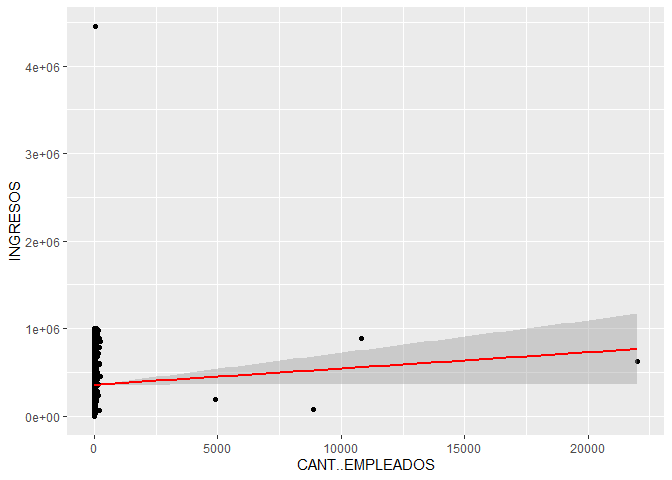
\includegraphics{Tarea-Betamétrica_files/figure-latex/unnamed-chunk-4-1.pdf}

\begin{Shaded}
\begin{Highlighting}[]
\CommentTok{\# Prueba de autocorrelación}
\NormalTok{modelo\_corr }\OtherTok{\textless{}{-}} \FunctionTok{dwtest}\NormalTok{(modelo) }
\FunctionTok{print}\NormalTok{(modelo\_corr)}
\end{Highlighting}
\end{Shaded}

\begin{verbatim}
## 
##  Durbin-Watson test
## 
## data:  modelo
## DW = 1.6932, p-value < 2.2e-16
## alternative hypothesis: true autocorrelation is greater than 0
\end{verbatim}

\begin{Shaded}
\begin{Highlighting}[]
\CommentTok{\# Prueba de heterocedasticidad}
\NormalTok{bptest\_result }\OtherTok{\textless{}{-}} \FunctionTok{bptest}\NormalTok{(modelo)}
\FunctionTok{print}\NormalTok{(bptest\_result)}
\end{Highlighting}
\end{Shaded}

\begin{verbatim}
## 
##  studentized Breusch-Pagan test
## 
## data:  modelo
## BP = 0.10759, df = 1, p-value = 0.7429
\end{verbatim}

\begin{Shaded}
\begin{Highlighting}[]
\CommentTok{\# Respuesta}
\CommentTok{\# Por cada empleado se añade 18.45 en los ingresos, sin embargo, debido al bajísimo valor de R{-}squared, }
\CommentTok{\# o existe gran impacto del número de empleados para aumentar los ingesos.}
\CommentTok{\# el gráfico 1 muestra que no existe la relación lineal entre las variables.}
\CommentTok{\# autocorrelación}
\CommentTok{\# DW=1.69 no existe alta correlación entre las variables}
\CommentTok{\# heterocedasticidad}
\CommentTok{\# p es 0.7429, por lo que no hay suficiente evidencia para rechazar la hipótesis nula.}
\end{Highlighting}
\end{Shaded}

\hypertarget{realiza-el-mismo-ejercicio-del-enunciado-anterior-pero-para-pichincha.-en-este-caso-suxf3lo-reporta-los-resultados-y-la-explicaciuxf3n-de-los-coeficiente.}{%
\section{3. Realiza el mismo ejercicio del enunciado anterior, pero para
pichincha. En este caso, sólo reporta los resultados y la explicación de
los
coeficiente.}\label{realiza-el-mismo-ejercicio-del-enunciado-anterior-pero-para-pichincha.-en-este-caso-suxf3lo-reporta-los-resultados-y-la-explicaciuxf3n-de-los-coeficiente.}}

\begin{Shaded}
\begin{Highlighting}[]
\CommentTok{\# Directorio}
\FunctionTok{setwd}\NormalTok{(}\StringTok{"C:}\SpecialCharTok{\textbackslash{}\textbackslash{}}\StringTok{Users}\SpecialCharTok{\textbackslash{}\textbackslash{}}\StringTok{Richard}\SpecialCharTok{\textbackslash{}\textbackslash{}}\StringTok{Documents}\SpecialCharTok{\textbackslash{}\textbackslash{}}\StringTok{DOCS RICHARD}\SpecialCharTok{\textbackslash{}\textbackslash{}}\StringTok{Cursos}\SpecialCharTok{\textbackslash{}\textbackslash{}}\StringTok{2023 Reto betametrica}\SpecialCharTok{\textbackslash{}\textbackslash{}}\StringTok{Tarea Betamétrica/"}\NormalTok{)}
\CommentTok{\# Archivo}
\NormalTok{db\_r }\OtherTok{\textless{}{-}}\NormalTok{ openxlsx}\SpecialCharTok{::}\FunctionTok{read.xlsx}\NormalTok{(}\StringTok{"empresas\_HEBM18.xlsx"}\NormalTok{)}
\CommentTok{\# asginar datos filtrados a db\_r}
\NormalTok{db\_r\_fil\_P }\OtherTok{\textless{}{-}}\NormalTok{ db\_r }\SpecialCharTok{\%\textgreater{}\%} 
  \FunctionTok{select}\NormalTok{(PROVINCIA,INGRESOS,CANT..EMPLEADOS) }\SpecialCharTok{\%\textgreater{}\%} 
  \FunctionTok{filter}\NormalTok{(INGRESOS}\SpecialCharTok{\textgreater{}}\DecValTok{0} \SpecialCharTok{\&}\NormalTok{ CANT..EMPLEADOS}\SpecialCharTok{\textgreater{}}\DecValTok{0} \SpecialCharTok{\&}\NormalTok{ PROVINCIA}\SpecialCharTok{==} \StringTok{"PICHINCHA                                         "}\NormalTok{)}
\NormalTok{db\_r\_fil\_P1 }\OtherTok{\textless{}{-}}\NormalTok{ db\_r\_fil\_P }\SpecialCharTok{\%\textgreater{}\%} 
  \FunctionTok{select}\NormalTok{(INGRESOS,CANT..EMPLEADOS)}
\FunctionTok{summary}\NormalTok{(db\_r\_fil\_P1)}
\end{Highlighting}
\end{Shaded}

\begin{verbatim}
##     INGRESOS       CANT..EMPLEADOS  
##  Min.   :    120   Min.   :   1.00  
##  1st Qu.: 164474   1st Qu.:   4.00  
##  Median : 289015   Median :   6.00  
##  Mean   : 357058   Mean   :  10.24  
##  3rd Qu.: 493858   3rd Qu.:  10.00  
##  Max.   :2994430   Max.   :2509.00
\end{verbatim}

\begin{Shaded}
\begin{Highlighting}[]
\NormalTok{modelo\_P }\OtherTok{\textless{}{-}} \FunctionTok{lm}\NormalTok{(INGRESOS}\SpecialCharTok{\textasciitilde{}}\NormalTok{.,}\AttributeTok{data =}\NormalTok{ db\_r\_fil\_P1)}
\FunctionTok{summary}\NormalTok{(modelo\_P)}
\end{Highlighting}
\end{Shaded}

\begin{verbatim}
## 
## Call:
## lm(formula = INGRESOS ~ ., data = db_r_fil_P1)
## 
## Residuals:
##      Min       1Q   Median       3Q      Max 
## -1221454  -190986   -67949   135604  2635552 
## 
## Coefficients:
##                  Estimate Std. Error t value Pr(>|t|)    
## (Intercept)     352108.24    3068.54  114.75  < 2e-16 ***
## CANT..EMPLEADOS    483.54      68.68    7.04 2.12e-12 ***
## ---
## Signif. codes:  0 '***' 0.001 '**' 0.01 '*' 0.05 '.' 0.1 ' ' 1
## 
## Residual standard error: 237500 on 6321 degrees of freedom
## Multiple R-squared:  0.007781,   Adjusted R-squared:  0.007624 
## F-statistic: 49.57 on 1 and 6321 DF,  p-value: 2.12e-12
\end{verbatim}

\begin{Shaded}
\begin{Highlighting}[]
\CommentTok{\#ingresos = intercept +b * cant empleado +error}
\CommentTok{\#ingresos = 352108.24+483.54*cant empleados}

\CommentTok{\#Gráficos}
\NormalTok{grafico2}\OtherTok{=}\FunctionTok{ggplot}\NormalTok{(db\_r\_fil\_P1,}\FunctionTok{aes}\NormalTok{(CANT..EMPLEADOS,INGRESOS))}
\NormalTok{grafico2}\SpecialCharTok{+}\FunctionTok{geom\_point}\NormalTok{()}\SpecialCharTok{+}\FunctionTok{geom\_smooth}\NormalTok{(}\AttributeTok{method =} \StringTok{"lm"}\NormalTok{,}\AttributeTok{colour=}\StringTok{"Blue"}\NormalTok{)}
\end{Highlighting}
\end{Shaded}

\begin{verbatim}
## `geom_smooth()` using formula = 'y ~ x'
\end{verbatim}

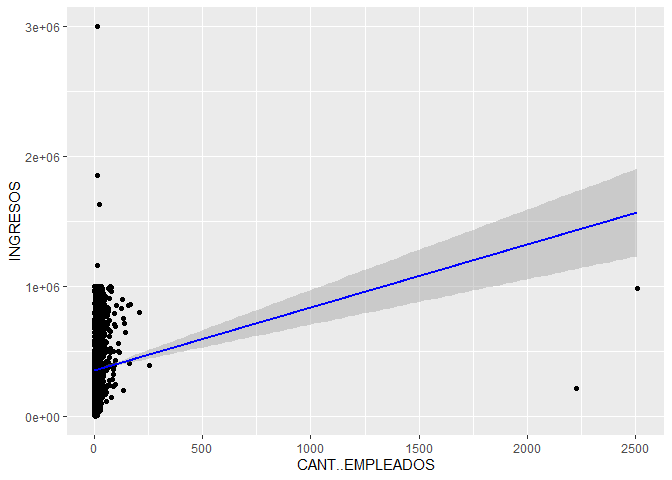
\includegraphics{Tarea-Betamétrica_files/figure-latex/unnamed-chunk-5-1.pdf}

\begin{Shaded}
\begin{Highlighting}[]
\CommentTok{\# Prueba de autocorrelación}
\NormalTok{modelo\_corr\_P }\OtherTok{\textless{}{-}} \FunctionTok{dwtest}\NormalTok{(modelo\_P) }
\FunctionTok{print}\NormalTok{(modelo\_corr\_P)}
\end{Highlighting}
\end{Shaded}

\begin{verbatim}
## 
##  Durbin-Watson test
## 
## data:  modelo_P
## DW = 1.5408, p-value < 2.2e-16
## alternative hypothesis: true autocorrelation is greater than 0
\end{verbatim}

\begin{Shaded}
\begin{Highlighting}[]
\CommentTok{\# Prueba de heterocedasticidad}
\NormalTok{bptest\_result\_P }\OtherTok{\textless{}{-}} \FunctionTok{bptest}\NormalTok{(modelo\_P)}
\FunctionTok{print}\NormalTok{(bptest\_result\_P)}
\end{Highlighting}
\end{Shaded}

\begin{verbatim}
## 
##  studentized Breusch-Pagan test
## 
## data:  modelo_P
## BP = 126.92, df = 1, p-value < 2.2e-16
\end{verbatim}

\begin{Shaded}
\begin{Highlighting}[]
\CommentTok{\# Respuesta}
\CommentTok{\# Por cada empleado se añade 483.54 en los ingresos, sin embargo, debido al bajísimo valor de R{-}squared, }
\CommentTok{\# no existe gran impacto del número de empleados para aumentar los ingesos.}
\CommentTok{\# A diferencia de Guayas, el número de empleados tiene mayor impacto en la generación de INGRESOS en Pichincha}
\CommentTok{\# el gráfico 1\_P muestra que no existe la relación lineal entre las variables.}
\CommentTok{\# autocorrelación}
\CommentTok{\# DW=1.54 no existe alta correlación entre las variables}
\CommentTok{\# heterocedasticidad}
\CommentTok{\# No hay suficiente evidencia para rechazar la hipótesis nula.}
\end{Highlighting}
\end{Shaded}


\end{document}
